\documentclass[class=article, crop=false, draft=true]{standalone}
\usepackage{graphicx}
\graphicspath{{../Figures}}

\usepackage{amsmath}

\usepackage{cleveref}

\begin{document}
%equations, bib. \\
\section{Previous project work}
This report is in a way a continuation of a specialization project\cite{specialization} done previously. The specialization project was focused on setting up a framework to work with. Part of hte specialization project has been starting work on a simulator that can be used to work on a control system. The control system is currently rudimentary implemented but there is room for improvement. The goal of the development for the conttrol sytemis to have it be platform agnostic. That is, the control system does not care whether tis' connected to a simulator or a vessel in hte real world. TThe way this is ideally implemented is by using ROS2. ROS2 is a framework to control robotics, built around publishers and subscribers that all act around topics.



\section{State of the Art}
\subsection{Physical issues}
\subsection{Simulation issues}

\section{Mathematical basis}

\section{Modelling and Control Design}

\begin{figure}
    \centering
    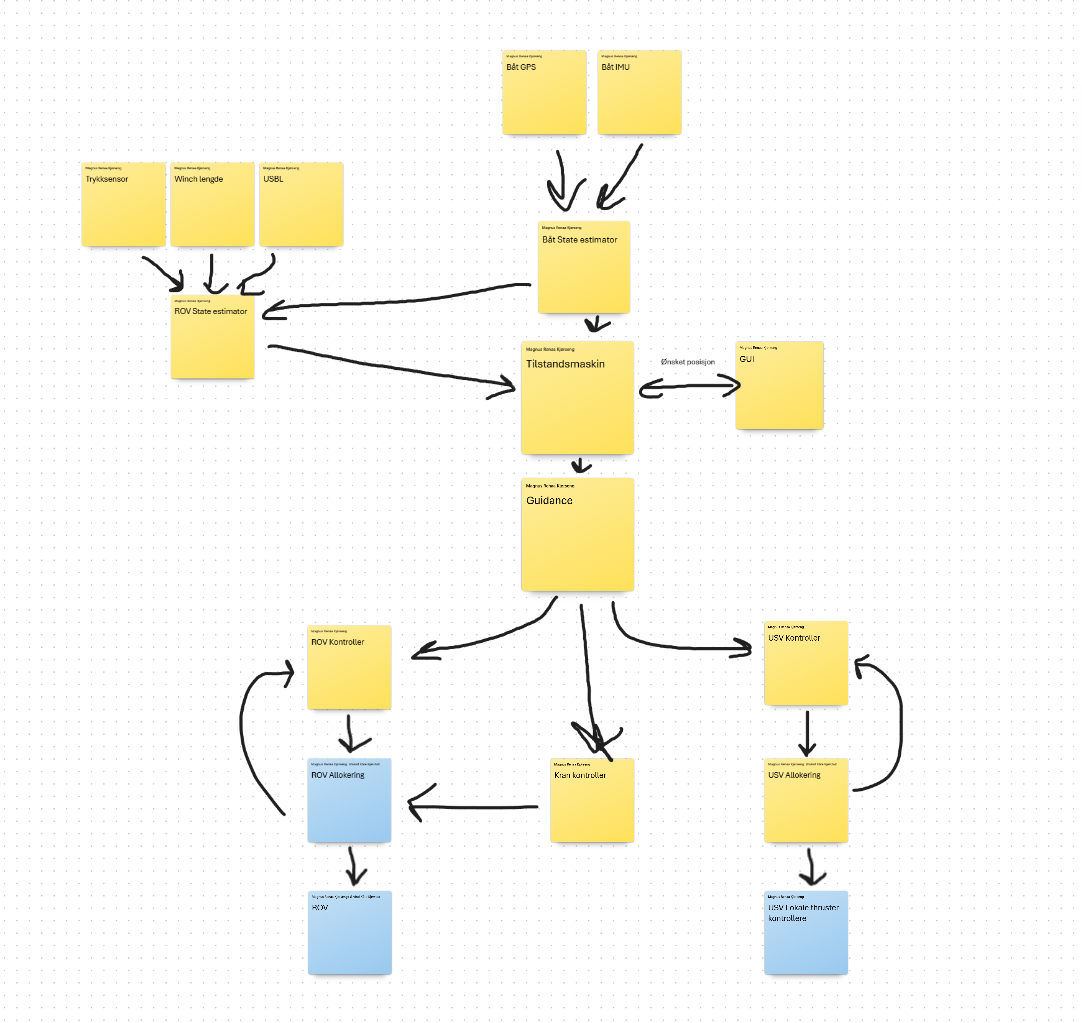
\includegraphics[width=0.9\textwidth]{control-system}
    \caption{A sketch of the control system design. TODO: Fiks bedre illustrasjon}
    \label{fig:control-system}
\end{figure}

\section{Sensorics}
The first step to knowing where to go is knowing where you are.

Alternatives for underwater navigation
\subsection{GNSS}
Only used above water
\subsection{Taut-wire positioning}
Mention taut wire, how it is usable somewhat btu not really because the ROV is not heavy enough to have the wire taut
\subsection{USBL}
Available and accurate

Need to consider limitations of accuracy of USBL re: salinity, water temperature/density, etc.

\section{State estimation}
The state estimator takes in the various sensor data and builds a single model of position. This is done because different sensors might have different accuracies or update times. The state estimator handles these discrepancies and builds a cohesive model. The state estimator feeds this more accurate position into the guidance system (TODO: Spørre øivind om det er guidance eller state machine som får posijonen. State machine skal jo bare være et informasjonslager?)

\section{State machine}
The state machine keeps track of variables for the total control system. These include current position, but also things like desired position or operating mode, gathered from the GUI.

\section{GUI}
The GUI is where a human operator interfaces with the control system. The GUI is supposed to include a position input for the surface vessel, mode switching between USV-Master, ROV-Master and idle/standby modes, along with other functions.

\section{Guidance}
The guidance system provides finer control of the vessel than what would be achieved by a state machine and controller alone. For instance it smooths acceleration/deceleration of the vessels by providing imaginary set points between the current position and the actual set point.

\section{Controller}
The controller finds a desired force input based on the difference (error) between the current position and the desired position. The current implementation uses a simple PID for this. This force input is fed forward to the allocator.

The shape of the force coming out of the controller is as \[\tau = \begin{bmatrix}X \\ Y \\ N\end{bmatrix}\]

\section{Allocation}
The allocator works like a translation layer between the controller and the local controllers. The controller provides a force input on the vessel's center of gravity. By inputting forces on the center of gravity, no torques are produced from lateral forces, nor lateral forces from the torque.

In abstract terms, the allocator finds and applies a transformation matrix \(T\) such that \[Tf = \tau\] where \(f\) is a vector of vectors with the lateral forces for each thruster. For this case with two thrusters, it will look something like \[f = \begin{bmatrix}x_1 \\ y_1 \\ x_2 \\ y_2 \end{bmatrix}\]
The transformation matrix can be written explicitly for the USV, since it has a very simple thrust configuration. For larger configurations it might be better to write each thruster's transformation individually and either add or remove them depending on the type of move necessary (larger moves use only larger thrusters etc.).
\begin{equation}\label{eq:transform_matrix}
T = \begin{bmatrix}1 & 0 & 1 & 0 \\ 0 & 1 & 0 & 1 \\ -l_{y_1} & l_{x_1} & -l_{y_2} & l_{x_2}\end{bmatrix}
\end{equation}

\begin{figure}
    \centering
    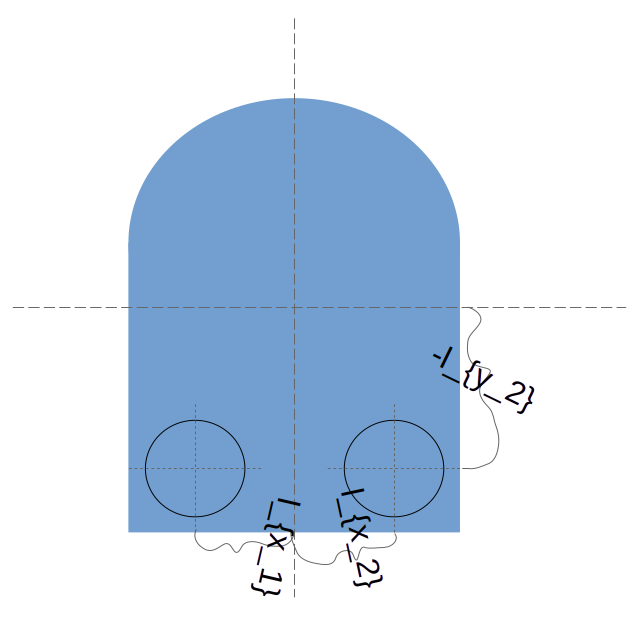
\includegraphics[width=0.9\textwidth]{thruster_position_sketch}
    \caption{Sketch of how the thruster position values in \cref{eq:transform_matrix} are found. The thruster configuration will be input to the allocator through a config file.}
    \label{fig:thruster_position_sketch}
\end{figure}

Since \(\tau\) and \(T\) are known, we can find \(f\) by performing a pseudoinverse on \(T\) leading us to the equation

\begin{equation}\label{eq:final_allocator}
f = T^\dagger \tau
\end{equation}

where \(T^\dagger\) is the pseudoinverse of \(T\).

This can also be written longform as

\begin{equation}\label{eq:long_allocator}
\begin{bmatrix}x_1 \\ y_1 \\ x_2 \\ y_2 \end{bmatrix} = T^\dagger \begin{bmatrix}X \\ Y \\ N\end{bmatrix}
\end{equation}

The full matrix for \(T^\dagger\) is omitted because the pseudoinverse of a non-square matrix tends to be large and ugly. It will only be handled by machine hands anyway, and as such doesn't matter right now.

The ROV has a built-in allocator which works well enough. The only issue with the ROV's allocator is that it's configured for a neutrally buoyant vessel. For this system we need to filter the vertical force component so the ROV only handles high-frequent/small-amplitude responses and the crane handles larger amplitudes and lower frequencies. This is also necessary because of elasticity in the lifting cable.

\section{Local control and physical response}
The vessel in this iteration has two thrusters. The ROV has a closed working solution and will not be considered here except for in the hypothetical. Each of these local controllers receive a two-component vector (or three-component in the case of the ROV) which instructs the controller what the desired thrust is. The azimuth thrusters on the USV are able to apply a force in one direction (parallel to the propeller axis), but they are able to vector this one-dimensional thrust using the azimuth ring.

\end{document}
